%\newpage
\section{Modeling uncertainty of ISRF near the GC} 
\lb{app:ISRF}

\begin{table*}
  \begin{center}
    \caption{\label{tab:CRe_syst} 
Spectra of CR electrons near the GC relative to the reference model based on the ISRF calculation of \cite{Porter:2008ve} used in GALPROP v54.1.
}
\begin{tabular}{| l |c|c|} % <-- Alignments: 1st column left, 2nd middle and 3rd right, with vertical lines in between
\hline
ISRF model & Relative normalization at 1 GeV  & Index \\
\hline
\cite{Porter:2008ve} & 1 & 2.71 \\ 
\cite{2017ApJ...846...67P} R12 & 0.59 & 2.61 \\ 
\cite{2017ApJ...846...67P} F98 & 1.16 & 2.71 \\ 
\cite{2017MNRAS.470.2539P} & 1.64 & 2.79 \\ 
 \hline
    \end{tabular}
  \end{center}
\end{table*}


\begin{figure*}[h]
\centering
\includegraphics[width=\twopic\textwidth]{plots/ISRF_comparison_ld}
\caption{Comparison of ISRF SEDs at the GC (see text for more details).}
\label{fig:isrfs}
\end{figure*}

In this appendix we discuss the uncertainty of the IC model of the gamma-ray emission at the base of the FBs 
related to modeling of the ISRF near the GC.
In order to estimate this uncertainty, we compare the ISRF model of 
\cite{Porter:2008ve} (available with the distribution of GALPROP v54.1),
the ISRF model of \cite{2017MNRAS.470.2539P},
and two ISRF models of \cite{2017ApJ...846...67P}: 
R12, based on \cite{2012A&A...545A..39R},
and F98, based on \cite{1998ApJ...492..495F}.
In Figure \ref{fig:isrfs} we show the corresponding densities of ISRFs averaged over the cylinder with the 
radius $R = 1.5$ kpc and the height $z = \pm 0.3$ kpc around the GC, which approximately corresponds 
to the latitude stripe $|b| < 2\degr$ and $|\ell| < 10\degr$.
We notice that there can be up to a factor of 2 differences in the ISRF energy density at the peak 
of the SL emission (around 1 $\mu$m) 
and an order of magnitude differences in the IR wavelengths (around 100 $\mu$m),
which can affect the inferred populations of CR electrons producing the IC gamma rays 
\citep[see also][]{2017ApJ...846...67P, 2019APh...107....1N}.


In Figure \ref{fig:GC_CR} we show the IC models of the gamma-ray emission 
at the base of the FBs in the rectangle $b \in (-2\degr, 2\degr)$, $\ell \in (-10\degr, 0\degr)$
for the different ISRF models near the GC.
We separate the SL, IR, and CMB contributions.
The SL and IR ISRFs are separated by splitting the radiation field energy densities at 0.1 eV ($\approx 12\ \mu$m).
We model the CR electrons spectra by a power-law function with an exponential cutoff.
We fix the cutoff at 1 PeV and fit the normalization and the spectral index by fitting 
the IC model to the \Fermi-LAT spectral points.
The corresponding parameters are presented in Table \ref{tab:CRe_syst}.
We use the \cite{Porter:2008ve} ISRF as the reference model and show the normalizations of the CRe spectra
relative to the reference model (the normalizations are determined at 1 GeV).
The overall spread in the normalizations is about a factor of 3,
while the overall variation of the index of the CRe spectra is less than about 0.2.


\begin{figure*}[h]
\centering
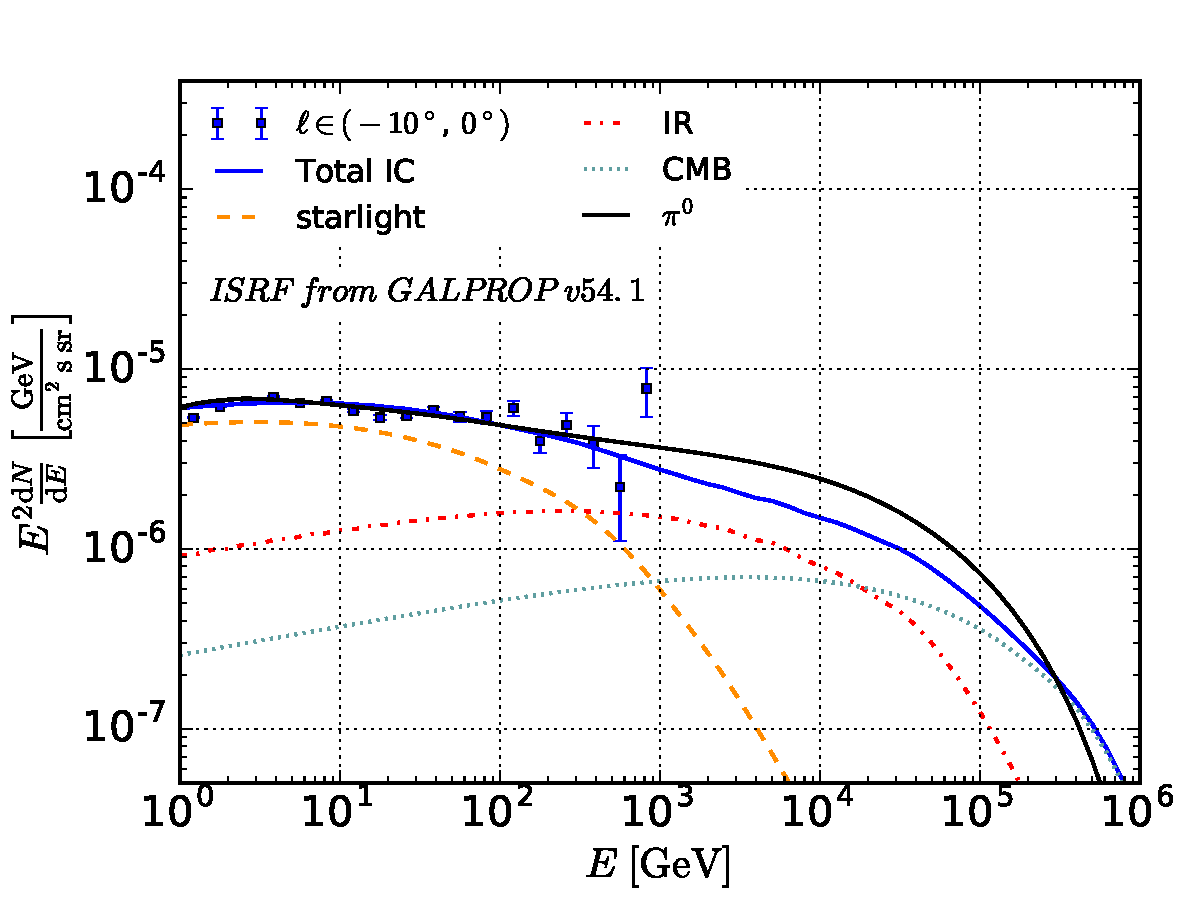
\includegraphics[width=\twopic\textwidth]{plots/SED_ISRF_componentsboxes_source_0_v54}
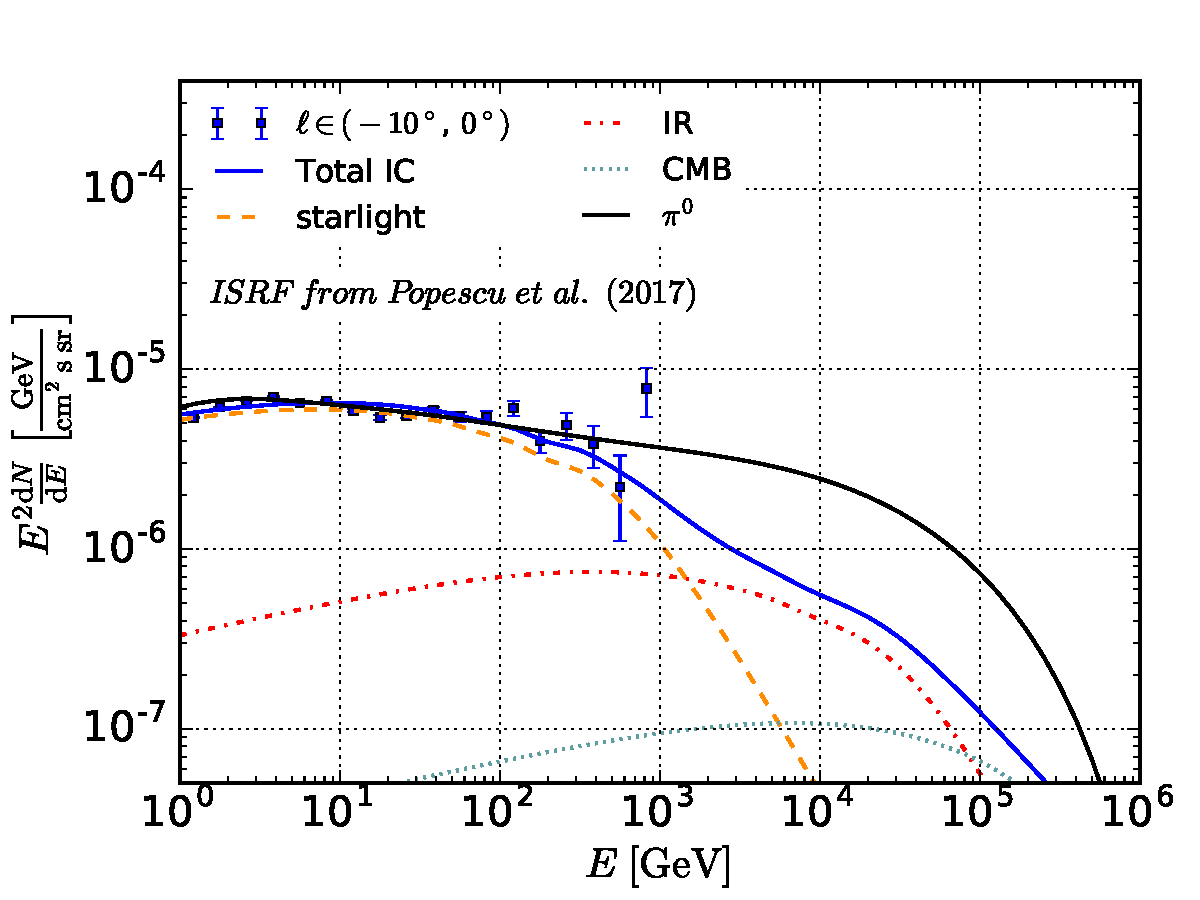
\includegraphics[width=\twopic\textwidth]{plots/SED_ISRF_componentsboxes_source_0_Popescu}
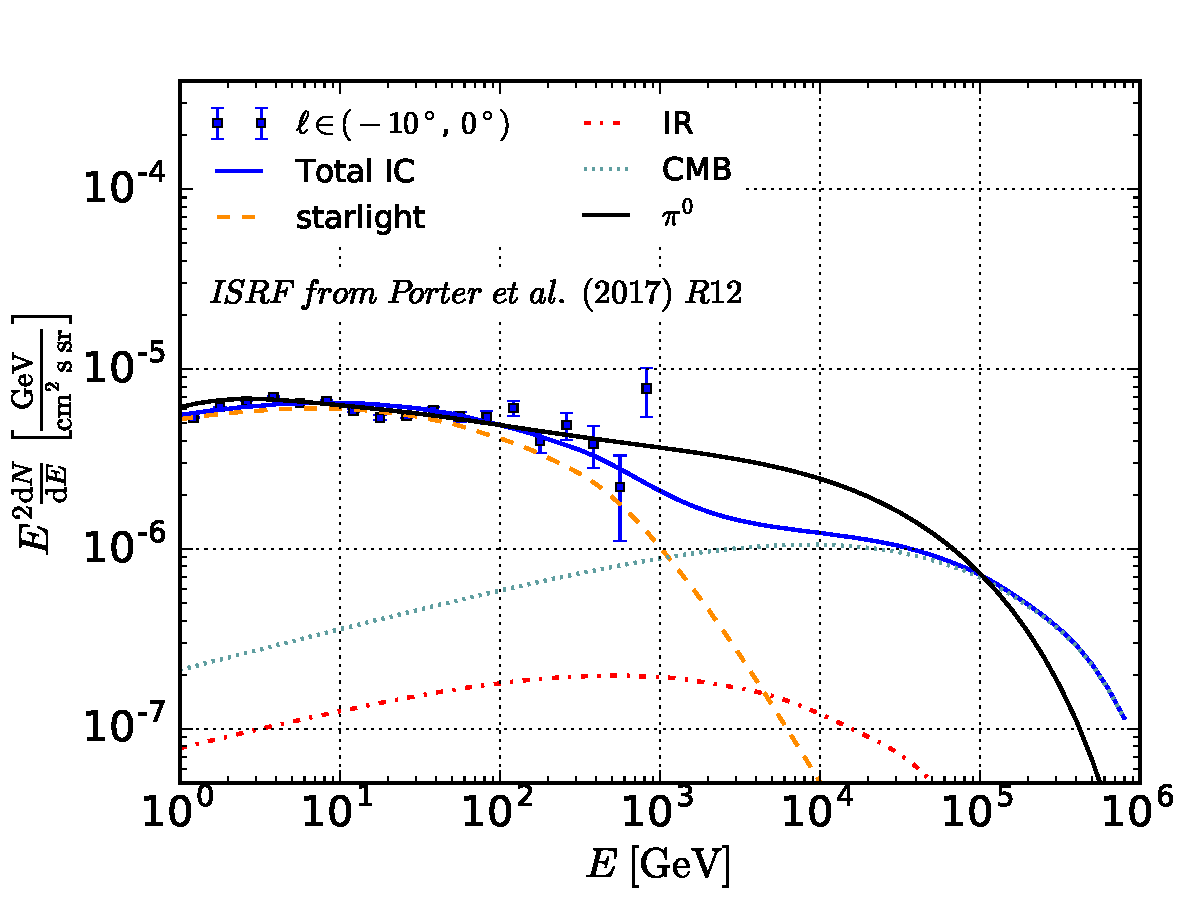
\includegraphics[width=\twopic\textwidth]{plots/SED_ISRF_componentsboxes_source_0_R12}
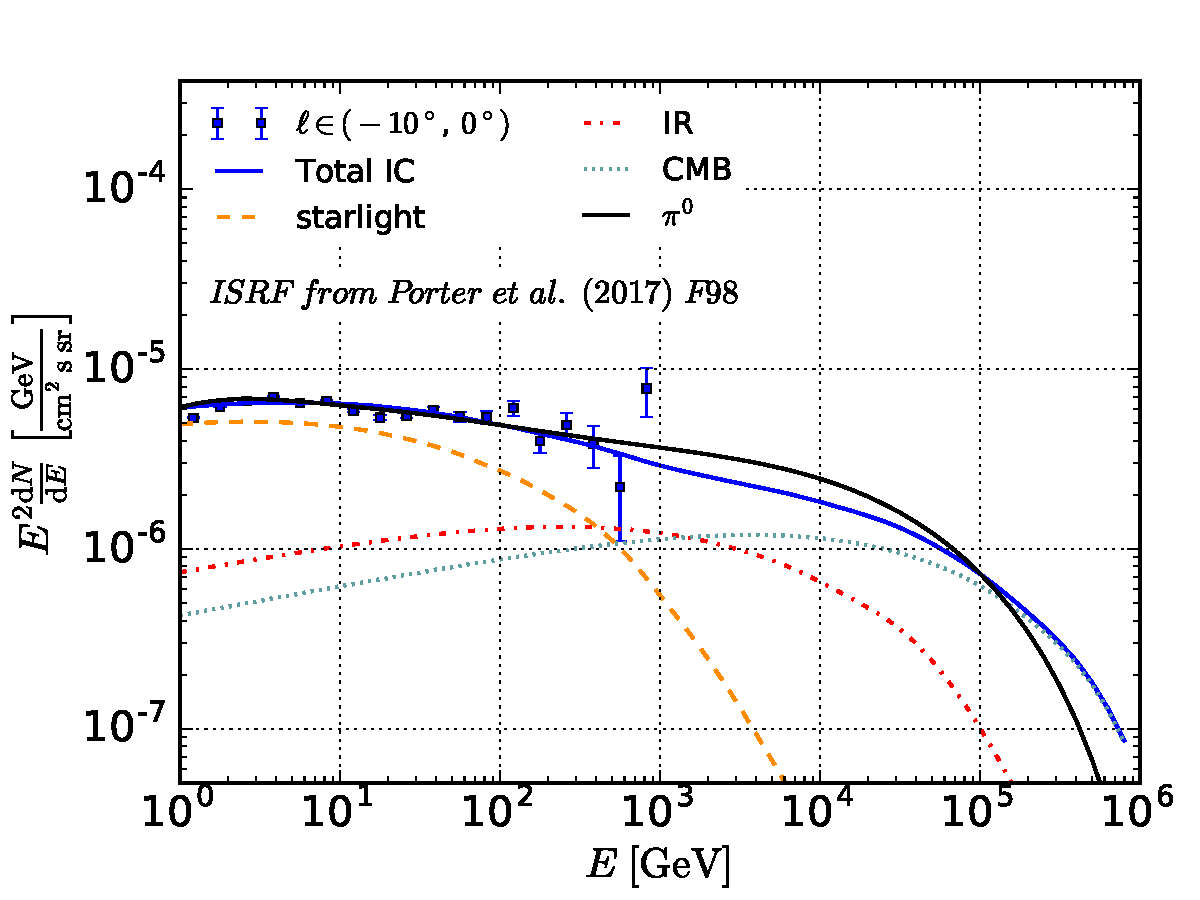
\includegraphics[width=\twopic\textwidth]{plots/SED_ISRF_componentsboxes_source_0_F98}
\caption{Contribution of different components of ISRFs to the IC model of the gamma-ray emission.
The data points correspond to the emission at the base of the FBs in the rectangle $b \in (-2\degr, 2\degr)$, $\ell \in (-10\degr, 0\degr)$
(middle panel in Figure \ref{fig:SED_with_fits}).
The spectrum of CR electrons is modeled as a power-law function with an exponential  cutoff at 1 PeV.
We separate the SL and the IR contributions to the ISRF by formally splitting the ISRF at 0.1 eV.}
\label{fig:GC_CR}
\end{figure*}




